%----------------------------------------------------------------------------
\chapter{GraphWalker}\label{sect:GraphWalker implementation of Garage Gate model}
%----------------------------------------------------------------------------
\section{GraphWalker}
%----------------------------------------------------------------------------

GraphWalker is a open source Model-based testing tool for test automation. It's designed to make it easy to design your tests using directed graphs. The tool generates test paths from these given graphs, which could be connected to each other. Each graph will have it's own set of generator(s) and stop condition(s). A path is used to call the corresponding methods or functions of your SUT (system under test). An edge in the directed graph represent an action in the system, consequently a vertex means a verification state, where we can check assertions in code. 


There are two ways to execute GraphWalker:
\begin{itemize}
	\item Offline: The path generation from the graph is done once (typically with command line), and these tests needs to be stored. A test automation system handle the tests. 
	\item Online: The path generation from the graph is created during the execution of the tests, run-time. If you have java coded SUT, it is pretty easy to add annotations to SUT and connect that to the generated paths.
\end{itemize}


\section{GraphWalker implementation in Eclipse}

 We can connect more models with the \textit{SHARED:someName} keyword in a vertex. Consequently I have created a yEd graph model for test scenarios for the garage gate state machine (see \figref{Garage Statemachine}), and a graph model for the lamp, which called from the previous graph.

\begin{figure}[!ht]
	\centering
	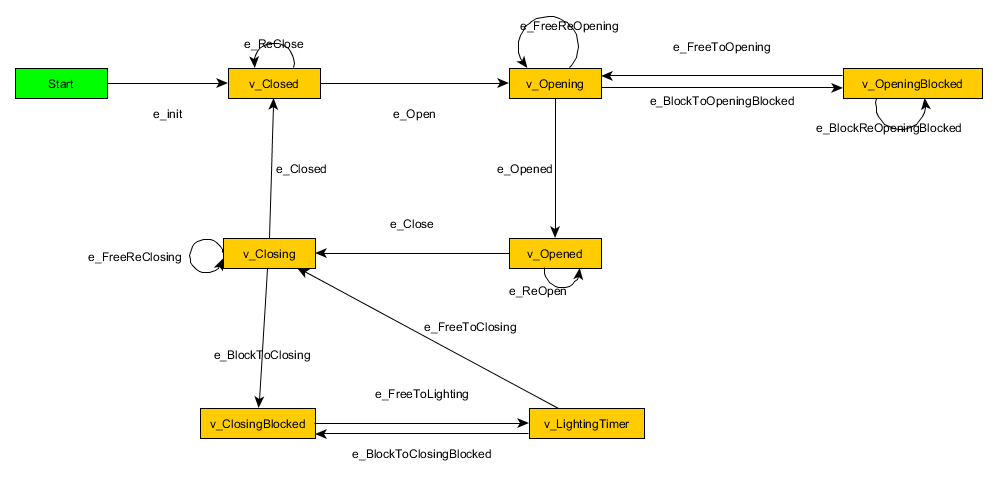
\includegraphics[width=150mm, keepaspectratio]{figures/GateModel.png}
	\caption{Garage gate model with yEd}
	\label{fig:GateModel}
\end{figure}

\begin{figure}[!ht]
	\centering
	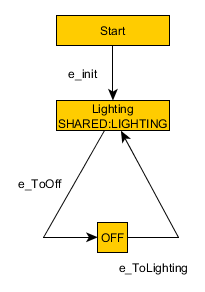
\includegraphics[width=50mm, keepaspectratio]{figures/LightingModel.png}
	\caption{Lamp0 model with yEd}
	\label{fig:GateModel}
\end{figure}


Generated test with option: @GraphWalker(start = "e\_init", value = "random(vertex\_coverage(100))"), and the result was:
[INFO] Result :
[INFO] 
[INFO] {
	"totalFailedNumberOfModels": 0,
	"totalNotExecutedNumberOfModels": 0,
	"totalNumberOfUnvisitedVertices": 0,
	"verticesNotVisited": [],
	"totalNumberOfModels": 2,
	"totalCompletedNumberOfModels": 2,
	"totalNumberOfVisitedEdges": 14,
	"totalIncompleteNumberOfModels": 0,
	"edgesNotVisited": [
	{
		"modelName": "GateModel",
		"edgeId": "e0",
		"edgeName": "e\_init"
	},
	{
		"modelName": "GateModel",
		"edgeId": "e3",
		"edgeName": "e\_Close"
	},
	{
		"modelName": "GateModel",
		"edgeId": "e10",
		"edgeName": "e\_FreeToOpening"
	},
	{
		"modelName": "GateModel",
		"edgeId": "e13",
		"edgeName": "e\_BlockReOpeningBlocked"
	}
	],
	"vertexCoverage": 100,
	"totalNumberOfEdges": 18,
	"totalNumberOfVisitedVertices": 9,
	"edgeCoverage": 77,
	"totalNumberOfVertices": 9,
	"totalNumberOfUnvisitedEdges": 4
}
